\section{Vistas - Diagrama de Objetivos y Requerimientos}
\subsection{Diagrama general}
En este diagrama se muestra cuáles son los objetivos más grandes del proyecto, que se desarrollan en el resto de los diagramas.
\begin{figure}[H]
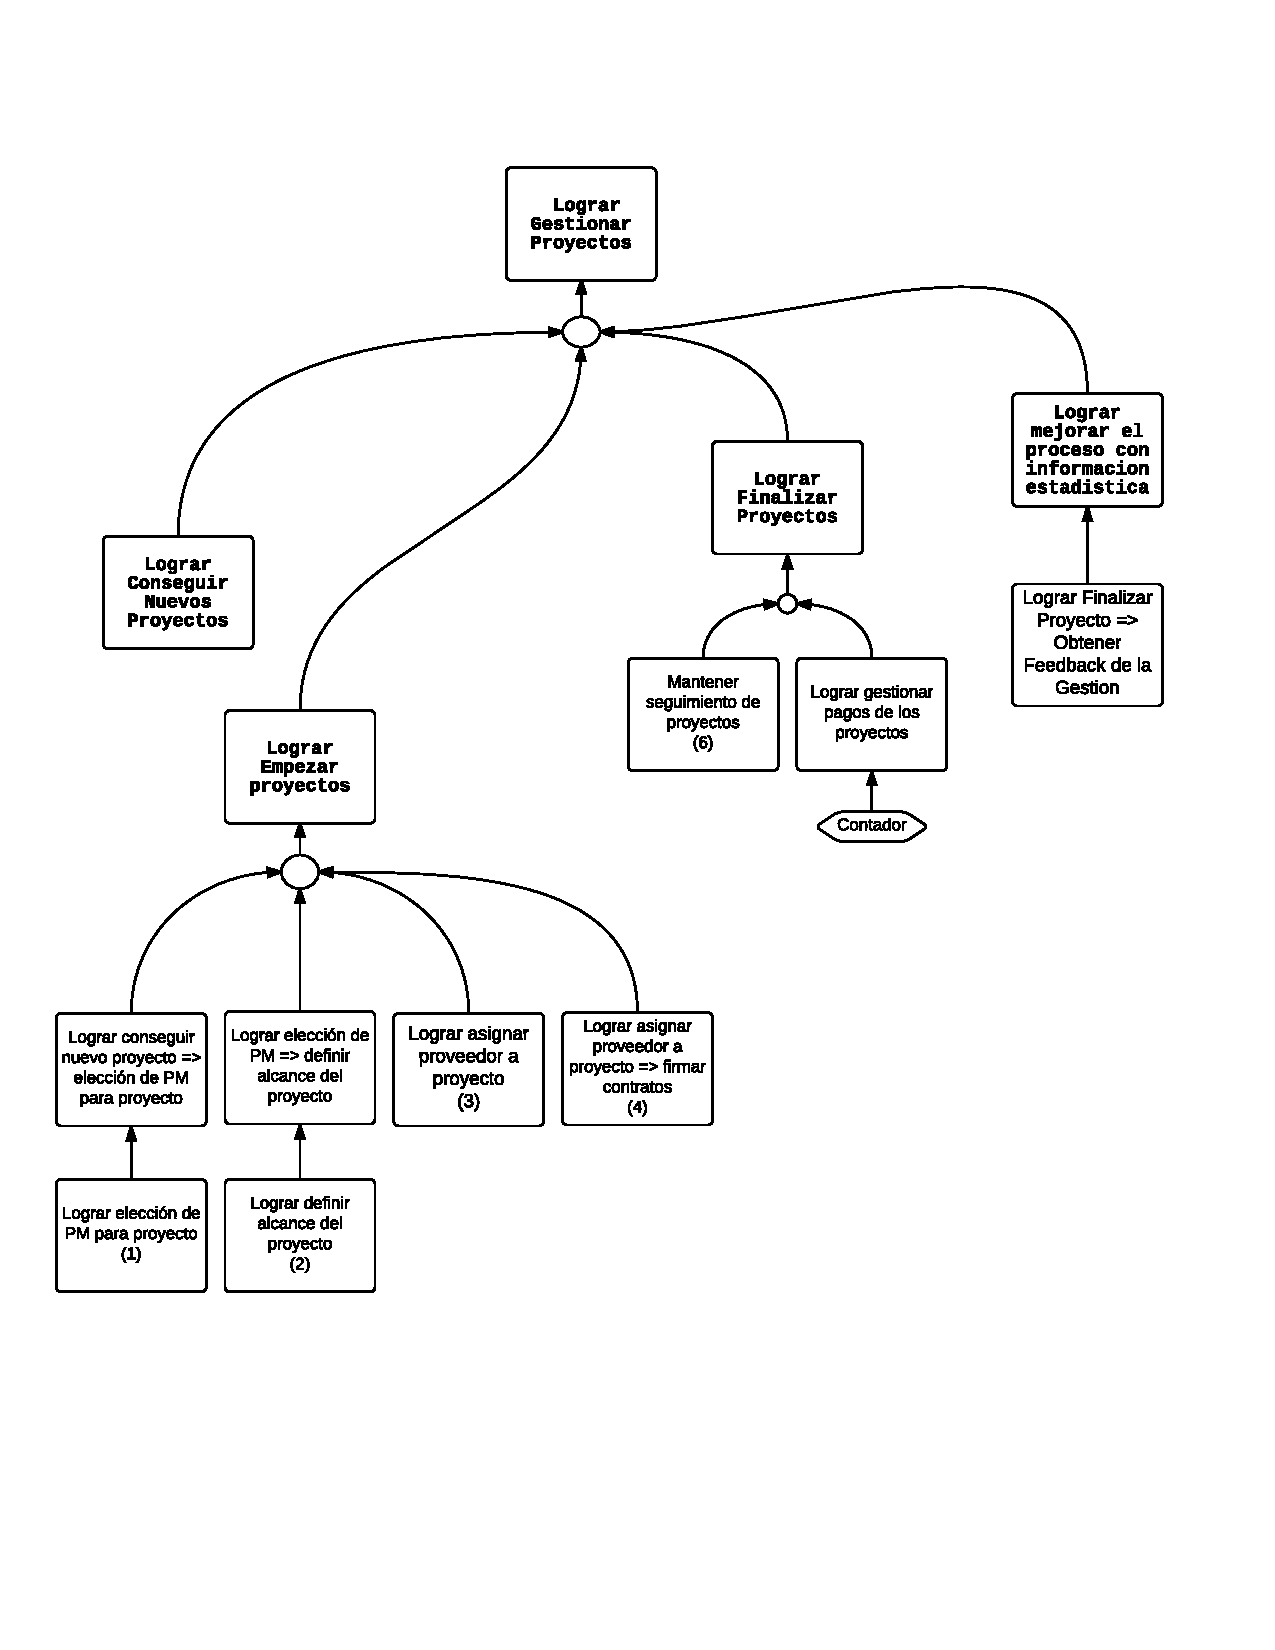
\includegraphics[width=\textwidth, clip=true, trim=15pt 170pt 15pt 80pt]{imagenes/objetivos/objetivos10.pdf}
\end{figure}
Podemos ver que los objetivos se dividen en los que permiten comenzar proyectos a partir de pre-proyectos, seguir proyectos en curso, conseguir nuevos proyectos (proveer herramientas para cargar preproyectos) y el circuito de feedback.

En particular el sistema de pagos no tiene que ver con el sistema, por lo tanto, no hay requerimientos de sistema que se vean en esta parte.

\newpage
\subsection{Lograr Comenzar Nuevos Proyectos}

Lograr comenzar un proyecto tiene varias etapas (comenzando con la entrada del preproyecto, hasta que los contratos están firmados y todo está listo para comenzar).
Las etapas son: Elección de PM, Definición de alcance, Asignación de Proveedor y Firma de contratos.

\begin{figure}[H]
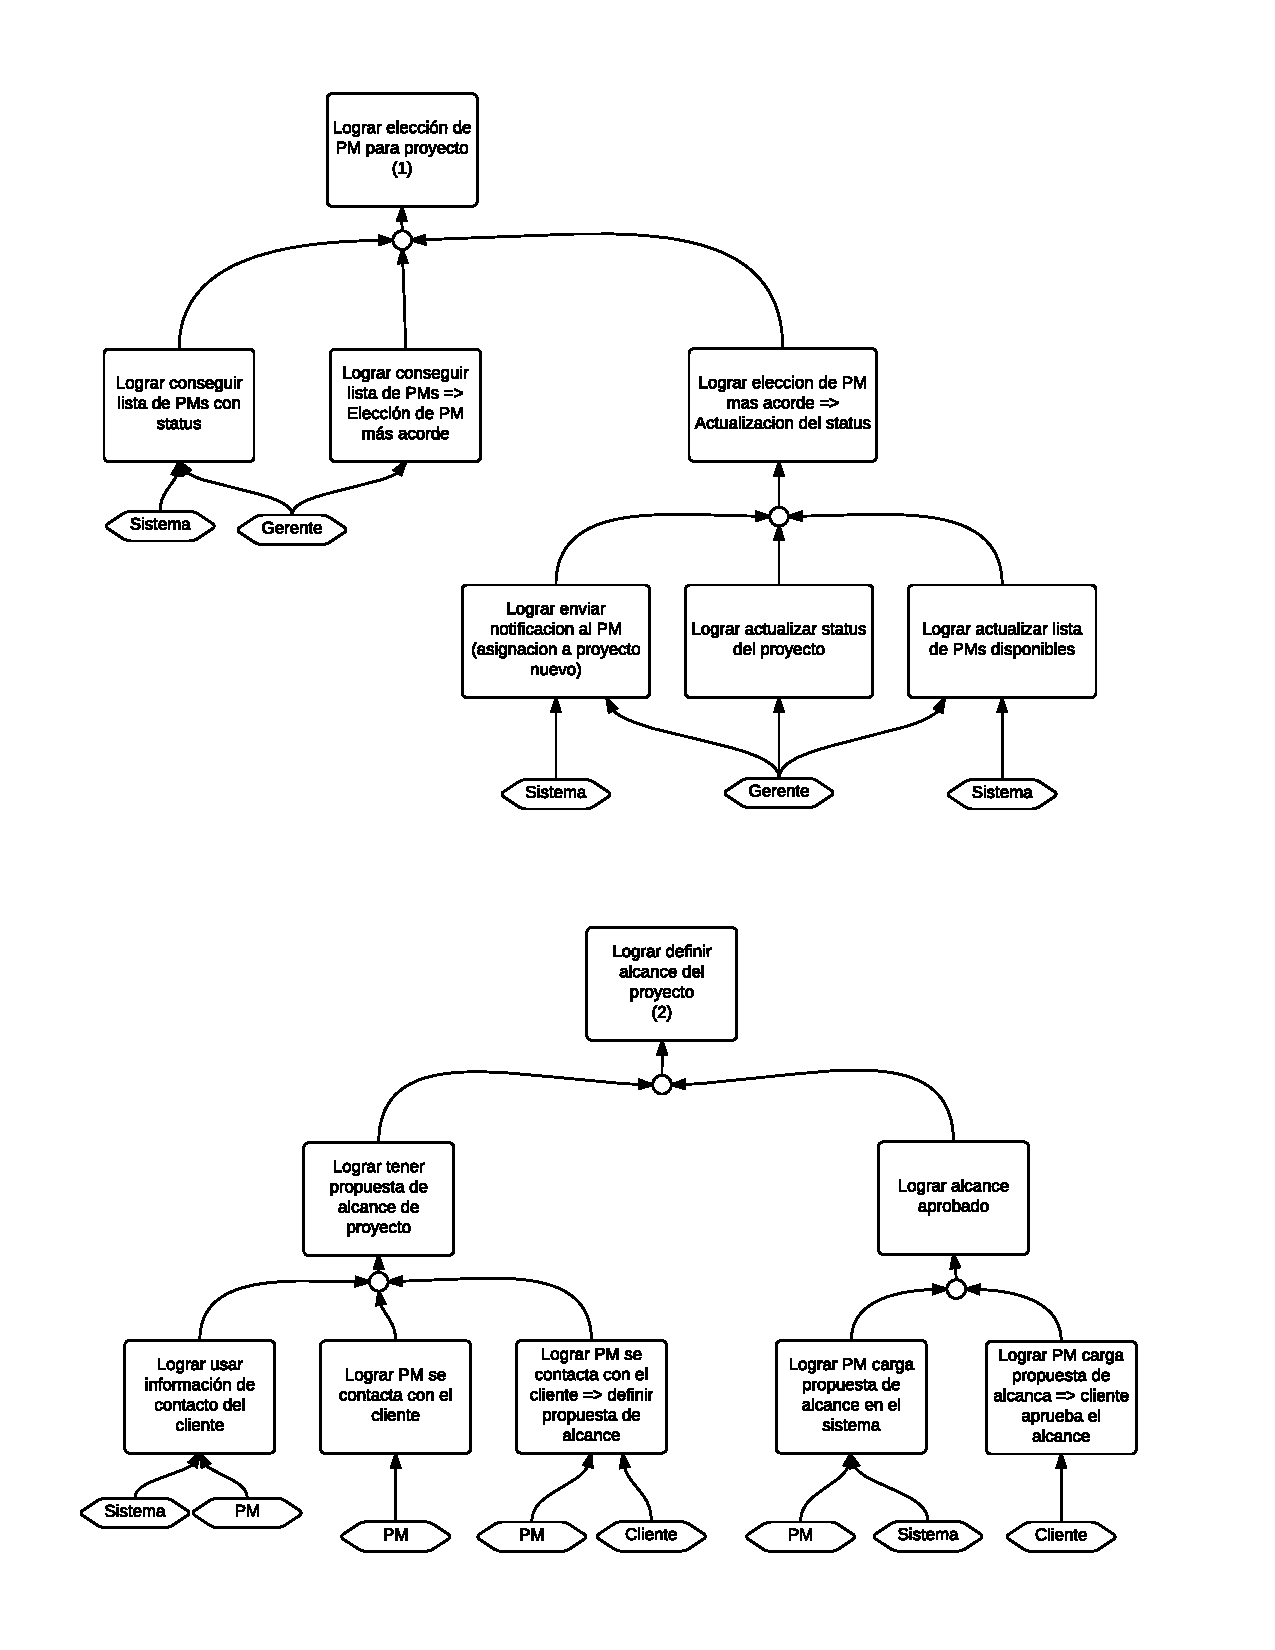
\includegraphics[width=\textwidth, clip=true, trim=15pt 30pt 15pt 40pt]{imagenes/objetivos/objetivos11.pdf}
\end{figure}

La elección de PM simplemente consiste en que el gerente pide una lista de PMs al sistema, asigna PM al proyecto, y el sistema notifica al PM.

\begin{figure}[H]
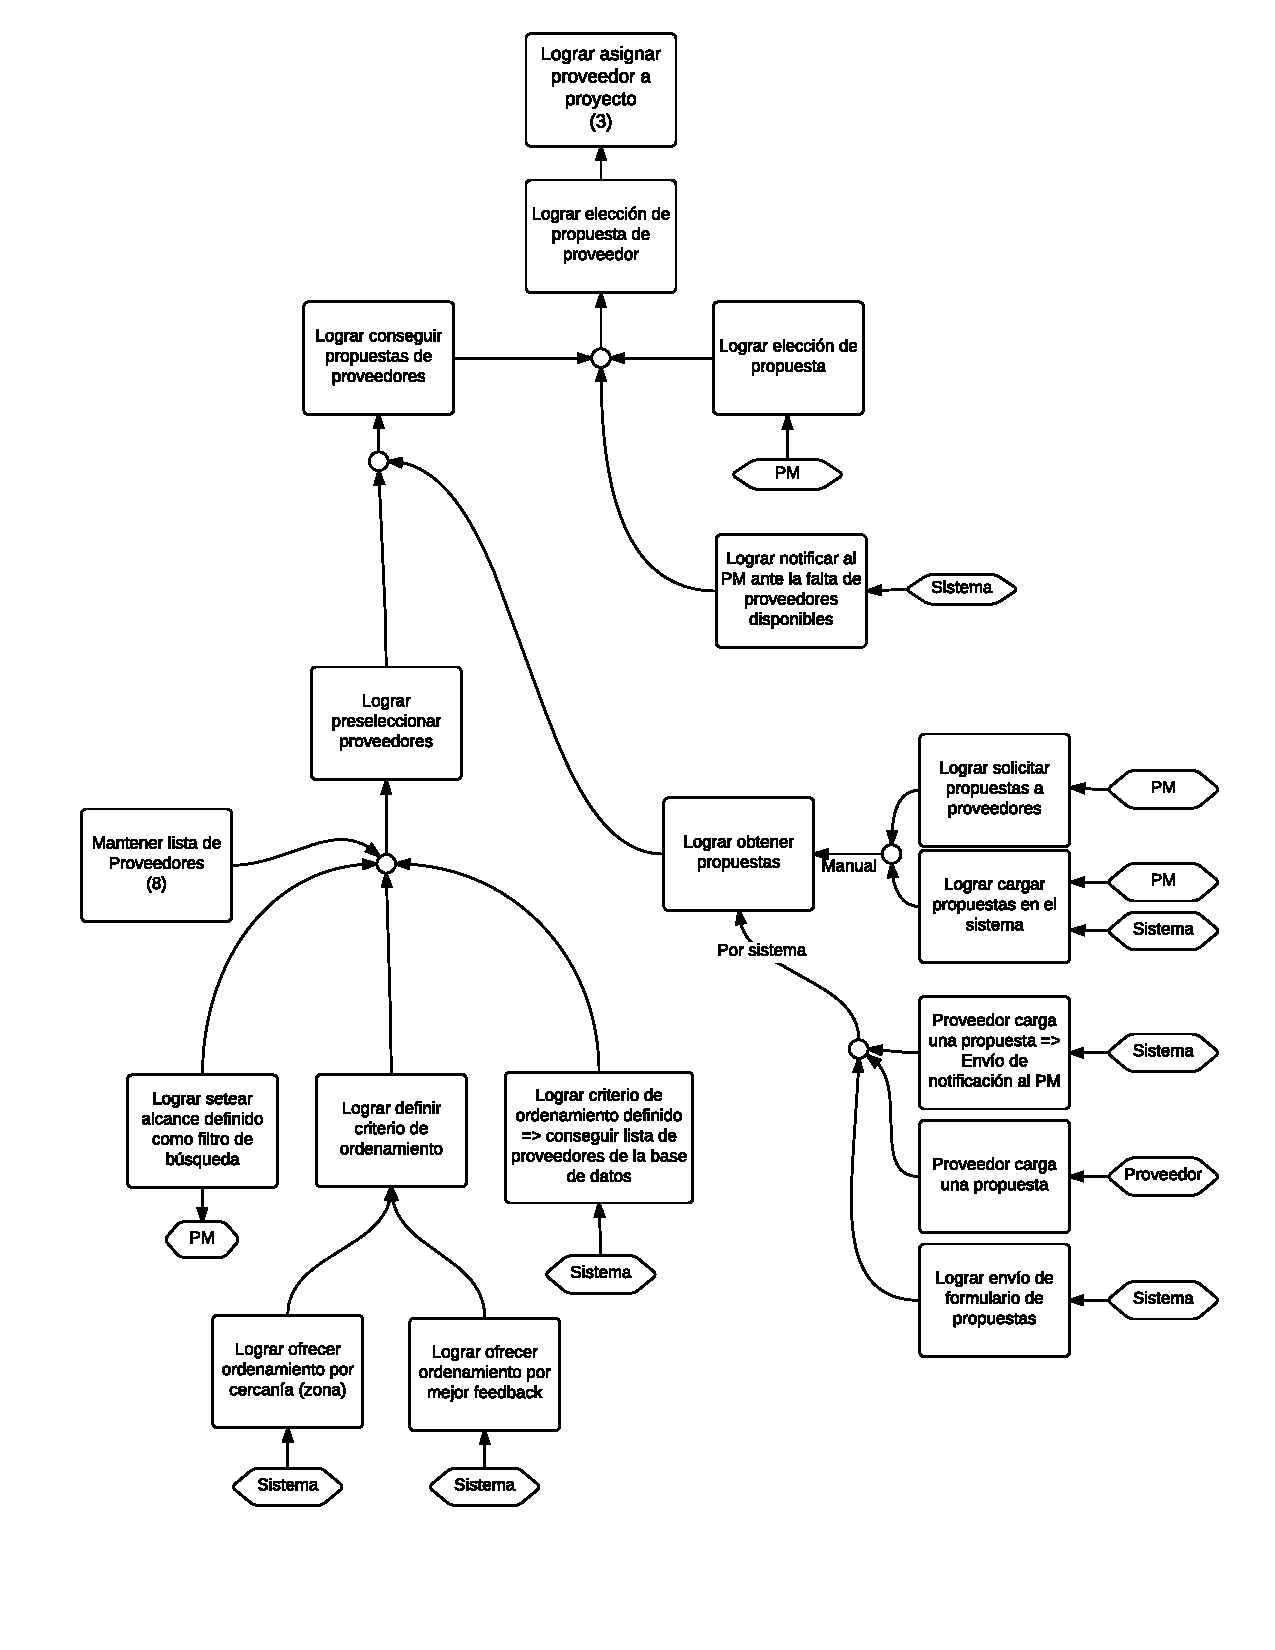
\includegraphics[width=\textwidth, clip=true, trim=15pt 50pt 15pt 0pt]{imagenes/objetivos/objetivos12.pdf}
\end{figure}

La asignación de proveedor consiste en que el PM consiga una lista de propuestas de proveedores y seleccione una.
El PM envía el alcance a los proveedores que cumplan con cierto criterio (puede elegir entre seleccionar los proveedores por zona o por puntaje) y espera las respuestas.

Los proveedores pueden cargar las propuestas en el sistema con un link de carga o mandarlas por mail y que el PM las cargue.

Esta parte depende de \textit{Mantener Lista de Proveedores}, que se detalla más adelante, y que es la tarea del Administrador.

\begin{figure}[H]
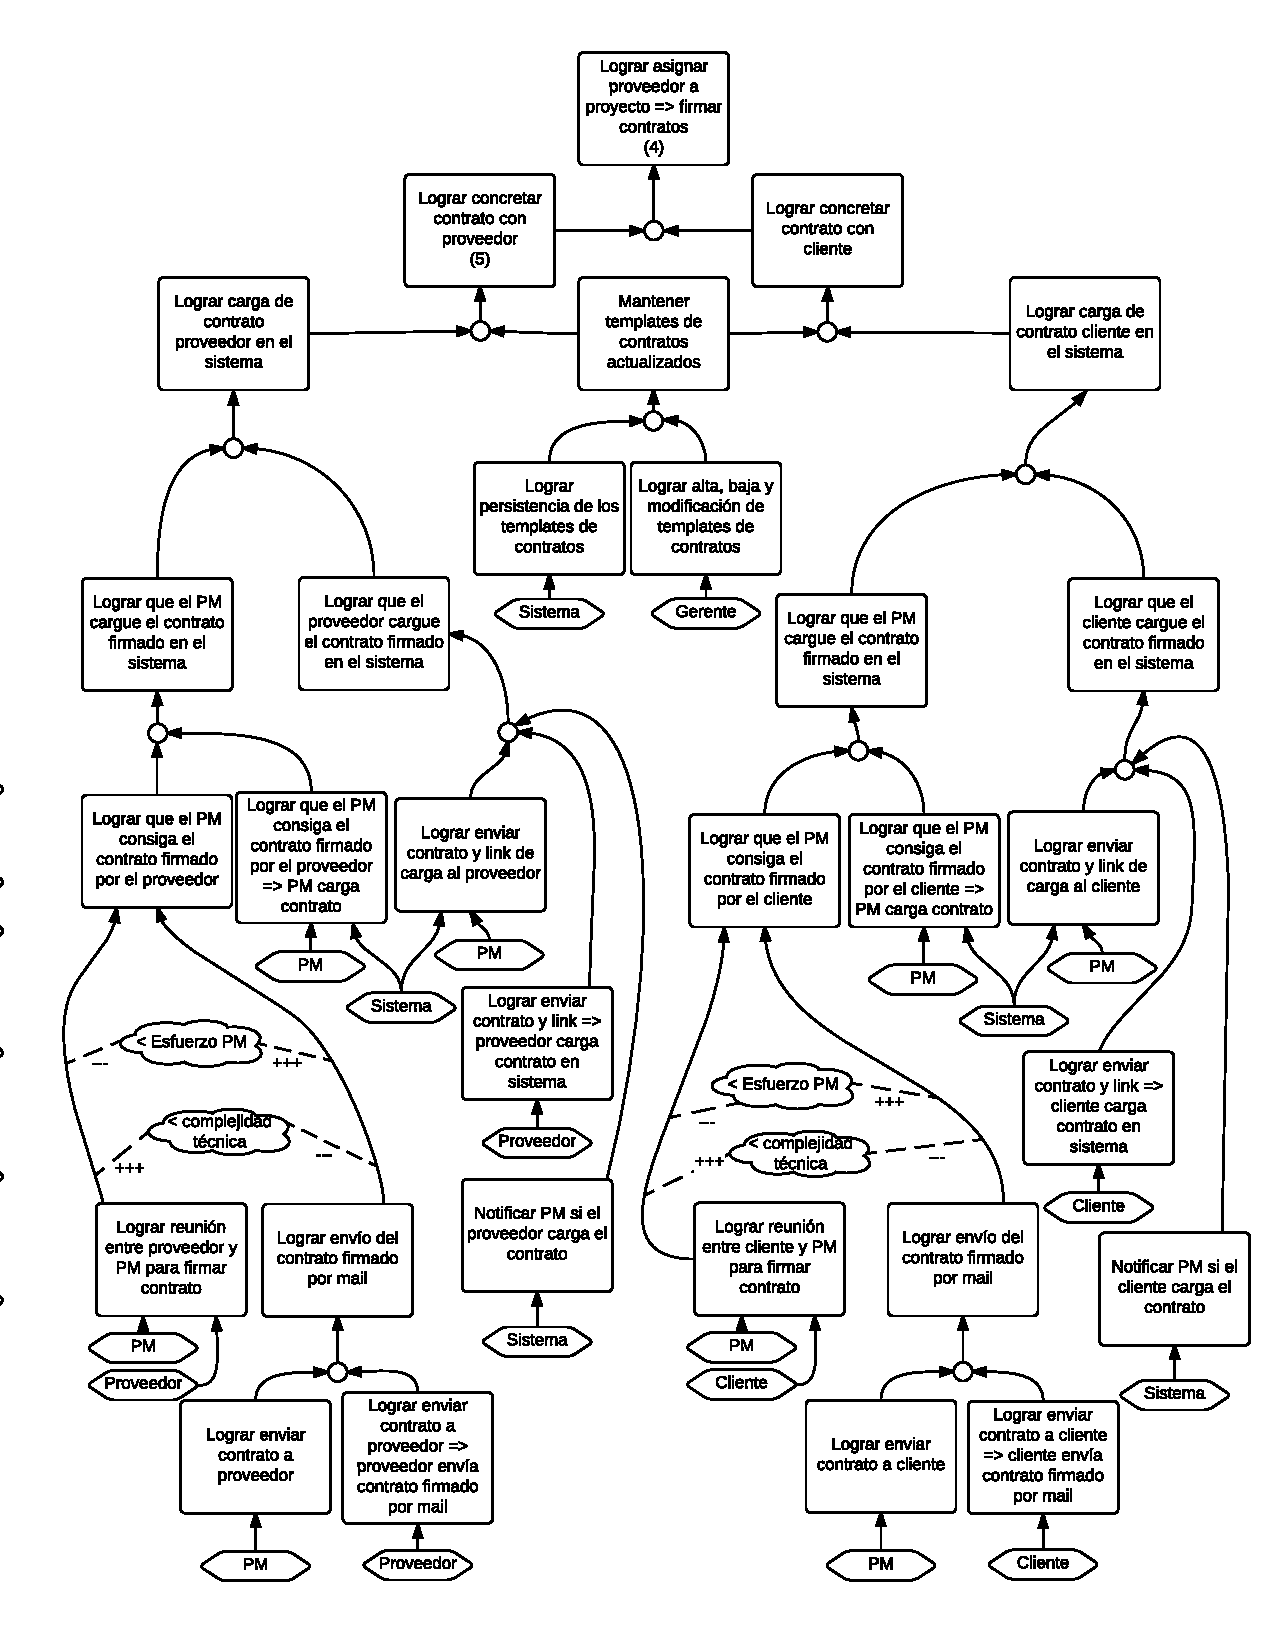
\includegraphics[width=\textwidth, clip=true, trim=15pt 30pt 12pt 20pt]{imagenes/objetivos/objetivos13.pdf}
\end{figure}

La firma de contratos depende del mantenimiento de templates actualizados (de dos tipos: proveedores y clientes), y de lograr la carga de ambos contratos en el sistema, con procedimientos similares en ambos casos.

Esto se puede conseguir tanto porque el PM cargue el contrato (como resultado de una reunión física o un envío por mail), o que el otro agente (cliente o proveedor en cada caso) utilice un link de carga para subir el contrato firmado, habiéndolo recibido por mail.
En caso de ocurrir esto, se notifica al PM que el contrato fue cargado.

\newpage
\subsubsection{Requerimientos de Sistema}
Los requerimientos para esta parte son:
\begin{itemize}
	\item En la asignación de PM:
	\begin{itemize}
		\item Ofrecer una lista de PMs con sus status
		\item Permitir al gerente asignar un PM a un proyecto
		\item Enviar notificaciones al PM al ser asignado a proyecto nuevo
		\item Actualizar lista de PMs disponibles
	\end{itemize}
	\item En la definición del alcance:
	\begin{itemize}
		\item Ofrecer información de contacto del cliente
		\item Ofrecer al PM cargar propuestas de alcance
	\end{itemize}
	\item En la asignación de proveedor:
	\begin{itemize}
		\item Dado un criterio de ordenamiento, ofrecer lista de proveedores más relevantes
		\item Implementar filtros por zona y por puntaje
		\item Notificar si no hay un proveedor disponible
		\item Ofrecer al PM cargar propuestas en sistema
		\item Ofrecer al proveedor cargar propuestas en sistema mediante link de carga
		\item Notificar al PM ante una carga de propuesta de un proveedor
	\end{itemize}
	\item En la firma de contratos:
	\begin{itemize}
		\item Almacenar y permitir al PM seleccionar templates para contratos.
		\item Proveer al PM mecanismos de carga de contratos (tanto para contratos de clientes como de proveedores).
		\item Proveer links de carga de contratos a proveedores y clientes
		\item Notificar al PM ante la carga de un contrato por parte de otro agente (cliente o proveedor).
	\end{itemize}
\end{itemize}

\newpage
\subsection{Seguimiento de Proyectos}
En esta parte nos aseguramos de poder resolver todos los problemas que surjan durante la ejecución de una obra en curso.
\begin{figure}[H]
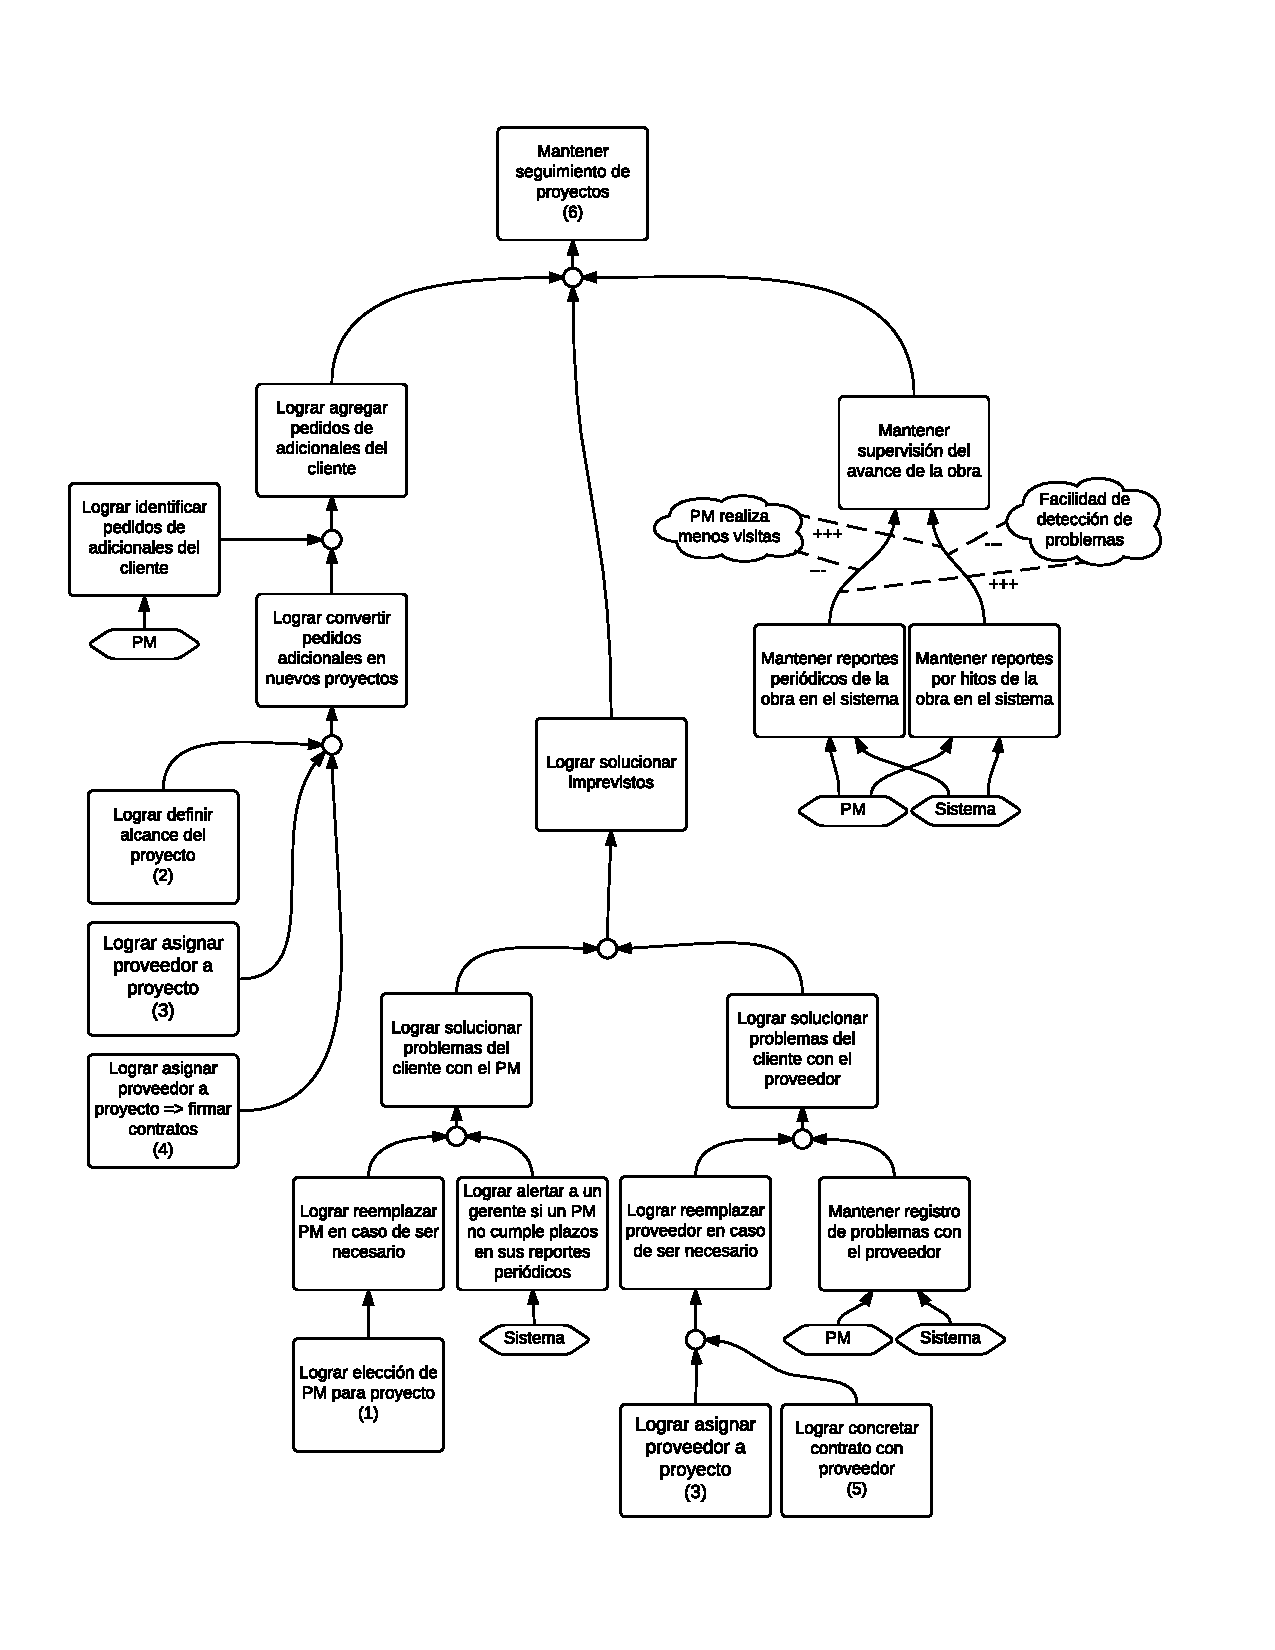
\includegraphics[width=\textwidth, clip=true, trim=15pt 50pt 15pt 60pt]{imagenes/objetivos/objetivos14.pdf}
\end{figure}

\newpage
Contempla la creación de adicionales (que son vistos como un nuevo proyecto con el mismo PM, por lo tanto depende de que se puedan realizar todas las etapas de creación de un nuevo proyecto a partir de la definición del alcance).

También contempla dos modos distintos de supervisión de obra (por hitos o periódicamente) con consideraciones de objetivos blandos que se analizarán más adelante.

Por último, se tiene el objetivo de solucionar imprevistos (irregularidades tanto del PM como del proveedor).
Para el PM, si no se cargan los reportes en los plazos establecidos, además, el gerente se notifica. En el caso del proveedor, se lleva un registro de irregularidades a cargo del PM, que los registra luego de sus visitas.

\subsubsection{Requerimientos de Sistema}
Los requerimientos para esta parte son:
\begin{itemize}
	\item Proveer interfaz al PM para cargar reportes de estado de proyectos.
	\item Alertar al gerente si un PM no carga sus reportes en los plazos establecidos.
	\item Mantener un registro de incidentes relacionados con el proveedor.
\end{itemize}

\subsection{Conseguir Nuevos Proyectos}
\begin{figure}[H]
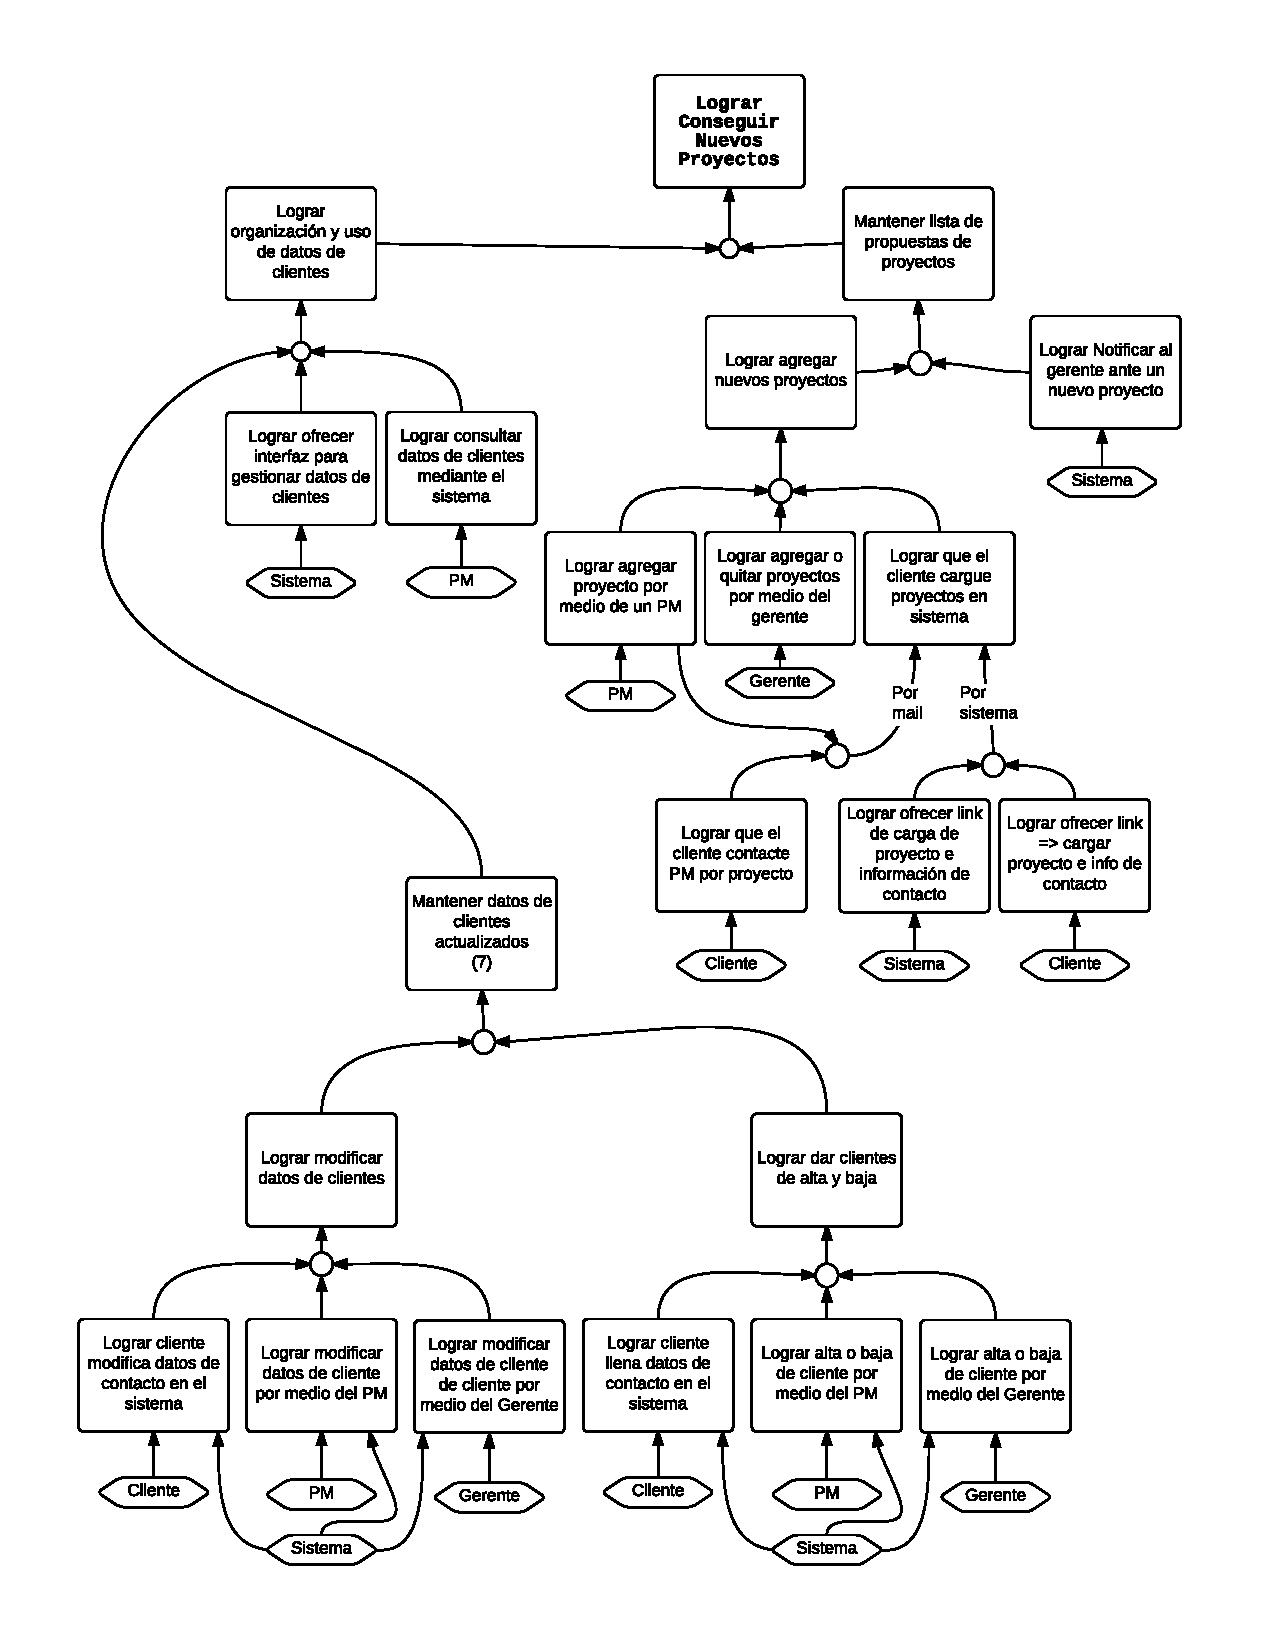
\includegraphics[width=\textwidth, clip=true, trim=15pt 20pt 15pt 20pt]{imagenes/objetivos/objetivos15.pdf}
\end{figure}

El objetivo de conseguir nuevos proyectos se logra sistematizando los datos de contacto de los clientes y las listas de pre-proyectos.

El sistema notifica al gerente ante la carga de un pre-proyecto.
Estos pueden ser agregados por un PM, gerente o cliente (que puede enviar por mail o por sistema su proyecto).

Tanto los PM como los gerentes pueden actualizar datos de clientes.
El cliente, cuando ingresa sus datos de contacto, puede ser contactado por un PM o gerente para terminar de llenar su ficha de datos.

Los requerimientos para esta parte son:
\begin{itemize}
	\item Ofrecer al cliente la opción de cargar un proyecto junto con su información de contacto.
	\item Sobre datos de clientes:
	\item Ofrecer al PM y Gerente la opción de cargar un proyecto con datos del cliente.
	\item Ofrecer una forma de visualizar y consultar datos de clientes.
	\item Ofrecer al PM y Gerente la posibilidad de dar de alta, de baja o modificar datos de clientes.
\end{itemize}

\subsection{Mantener Datos de Proveedores}
\begin{figure}[H]
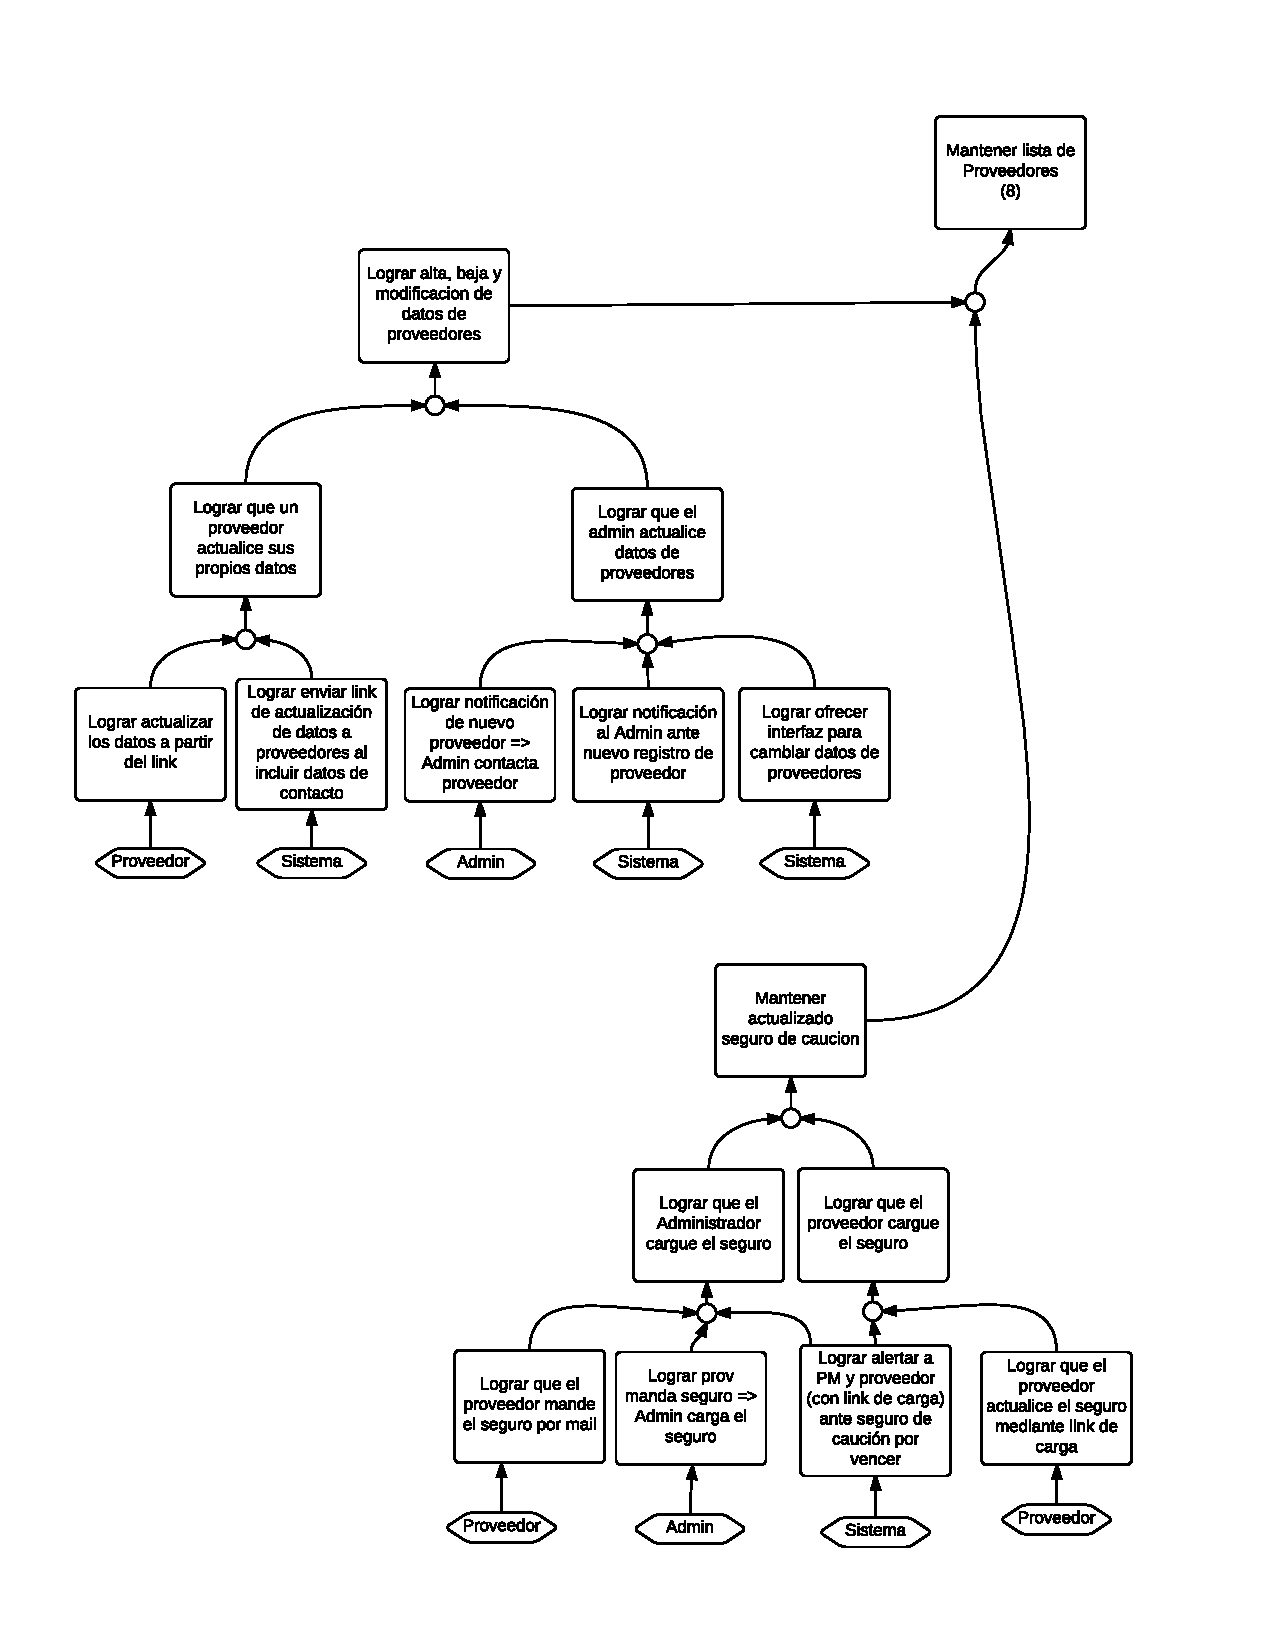
\includegraphics[width=\textwidth, clip=true, trim=15pt 40pt 15pt 40pt]{imagenes/objetivos/objetivos16.pdf}
\end{figure}

La tarea de mantener datos de proveedores tiene un encargado en sí misma: el Administrador.
Tiene dos tareas: la gestión de los datos de proveedores y el mantenimiento de los seguros de caución.

Cuando un nuevo proveedor se registra, se le envía un link para que termine de llenar sus datos.
Alternativamente, el Admin puede contactarlo (dado que se notifica ante un alta de proveedor) y pedirle sus datos para llenarlos él mismo.

Los seguros de caución siguen un esquema similar: ante el próximo vencimiento de un seguro, se envía una notificación con link de carga al proveedor para que lo actualice, y también se notifica al Administrador, que puede contactar al Proveedor y cargar el seguro él mismo si se lo envían por mail.

\subsubsection{Requerimientos de Sistema}

Los requerimientos para esta parte son:
\begin{itemize}
	\item Enviar un link a proveedores para completar su información dada la entrada de información de contacto.
	\item Notificar Admin ante el alta de un proveedor (datos de contacto).
	\item Permitir al Admin modificar datos de proveedores.
	\item Notificar Proveedor y Admin ante el próximo vencimiento de un seguro de caución.
	\item Enviar un link de carga de seguro de caución al proveedor, junto con la alerta.
	\item Permitir al Admin cargar un seguro de caución.
\end{itemize}

\newpage
\subsection{Feedback}
\begin{figure}[H]
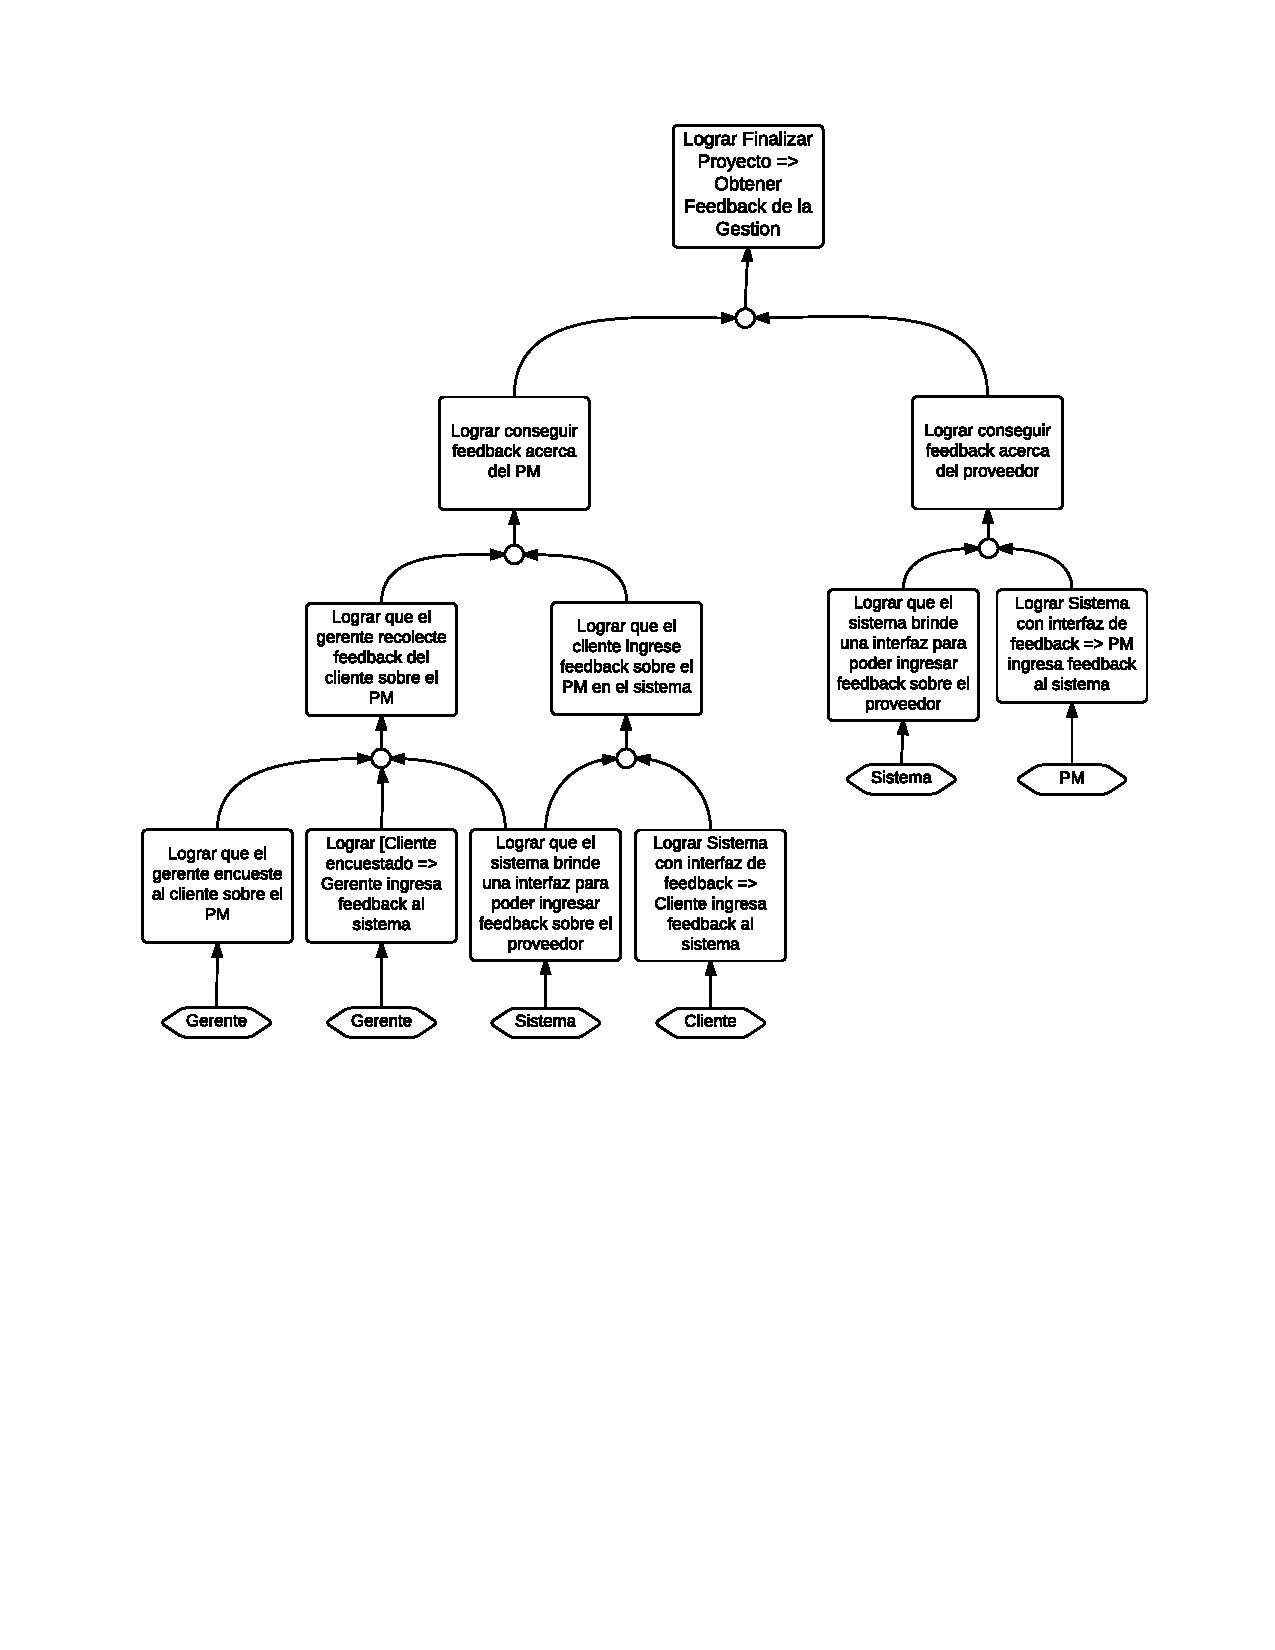
\includegraphics[width=\textwidth, clip=true, trim=15pt 290pt 15pt 40pt]{imagenes/objetivos/objetivos17.pdf}
\end{figure}

Se debe obtener Feedback del PM (llenado por el cliente) y del proveedor (llenado por el PM), para poder utilizarlo en los procesos del sistema.

Podemos confiar en que el PM cargue el Feedback porque es un empleado de la empresa.
En cambio para el cliente, se propone un curso alternativo en el que el gerente contacta al cliente, solicita el Feedback y lo carga en el sistema.

\subsubsection{Requerimientos de Sistema}
Los requerimientos para esta parte son:
\begin{itemize}
	\item Lograr ofrecer al PM la opción de completar Feedback sobre Proveedores.
	\item Lograr enviar al cliente una notificación con link de carga de Feedback sobre el PM.
	\item Lograr que el gerente ingrese Feedback del cliente respecto del PM al sistema.
\end{itemize}
